\documentclass[]{article}
\usepackage[backend=biber, style=apa]{biblatex}
\usepackage{paralist}
\usepackage{hyperref}
\usepackage{float}
\usepackage{graphicx}
\usepackage{booktabs}
\graphicspath{ {./images/} }

\addbibresource{researchProposal.bib}

\newtheorem{researchquestion}{RQ}

%opening
\title{Research Proposal \\
	A YOLOv8-based Analysis of Image Augmentation Techniques for Vehicle Detection in Adverse Weather Conditions}
	\author{
		Alexander Van Hecke \small(852631385) \and 
		Frederik Lefever    \small(838836963)}

\begin{document}

\maketitle

\begin{abstract}
	Vehicle detection is an important aspect of semi-automated traffic monitoring and surveillance.  We propose to investigate whether the technique of image augmentation can be used to increase the accuracy of vehicle detection in adverse weather conditions.  The study will evaluate whether the use of image augmentation to train a YOLO\small{v8} model increases accuracy compared to a baseline model.  We also propose to compare the effect of training with augmentated images to that of training with actual images of traffic in adverse weather conditions. To this extent we will train a YOLO\small{v8} model with actual images and compare with the same baseline model and the accuracy obtained from the first model. Our main hypothesis is that image augmentation can indeed be used to improve the accuracy of vehicle detection in adverse weather conditions. Our secondary hypothesis is that the accuracy of a model derived from augmented images falls within statistically insignificant margins when compared to a model obtained from actual images.  
\end{abstract}

\section{Introduction}

	Adverse weather conditions such as rainfall, snow and fog are widely considered to have an effect on traffic flow. Traffic breakdown occurs when demand exceeds capacity in some part of a transportation network and in \cite{stralenInfluenceAdverseWeather2015} it is shown that the odds of traffic breakdown at bottleneck locations are significantly increased by rainfall.  This can lead to considerable economic damage and provides a strong incentive to mitigate this problem as much as possible.
	
	Traffic monitoring and dynamic control of traffic flows can be part of a mitigation strategy. The current technology behind traffic monitoring uses vehicle detection in images captured from strategically placed CCTV cameras on highways. However, vehicle detection in images can be influenced by adverse weather conditions.
	
	Sometimes object detection can be improved with image augmentation techniques, in which the original images are rotated, shifted or mirror imaged to create a larger training set with more variability in the training images.	We propose to investigate the effect of image augmentation on the robustness of YOLO{\small v8}-based vehicle detection models. In particular, we propose to investigate the effect of artificially adding rain, fog and snow to real clear weather images of highways. Compared to augmentation by simple geometric transformations, the proposed kind of augmentation is thematic and focussed towards specific use cases. We expect to see a significant improvement of the mean intersection over union (IoU) for vehicle detection in models derived from YOLO{\small v8} by training on the augmented images. 
	
	We chose standard YOLO{\small v8} as a reference and base model to train from, because YOLO{\small v8} is state-of-the-art and comes pre-equipped with annotations for vehicle detection and many developer-convenience features. Also, YOLO{\small v8} is well-documented as a ready-to-use product and in scientific literature. Moreover, there is a large community around the YOLO models that can provide assistance should this be needed. Finally, YOLO{\small v8} is an open-source software, licensed under AGPL-3.0. All artifacts produced by the proposed study will hence be made available through a public GitHub repository.  
	
	The proposed research seeks to confirm the hypothesis that refining the standard YOLO{\small v8} with augmented images improves detection accuracy. We also try to confirm the hypothesis that such a model is ``as good as'' one trained from actual images of traffic in adverse weather conditions.

\section{Literature review}

	In the context of machine learning, image augmentation can broadly be defined as the automated creation of variation in actual image datasets. This technique can be used to avoid a learning algorithm overfitting the data. Overfitting occurs when a learning algorithm learns a function in such a way that it perfectly models the training data, but is unable to generalize beyond the training data. Large volumes of data with sufficient variation can alleviate the problem of overfitting. Yet sometimes sampling data from an application domain is nontrivial, eg. when learning from medical images.  Image augmentation can be used to artificially create additional images, or to add some sort of noise to images in order to make the resulting model more robust.
	
	A comprehensive survey of modern image augmentation techniques is presented in \cite{shortenSurveyImageData2019}. Several approaches such as geometric transformations, color space augmentations, kernel filters, mixing images, random erasing, feature space augmentation, adversarial training, generative adversarial networks, neural style transfer, and meta-learning, are explained. \cite{xuComprehensiveSurveyImage2023} offers a more recent survey of image augmentation techniques as used in deep learning. This survey introduces a novel taxonomy, where image augmentation algorithms are classified as either model-free, model-based, or optimizing policy-based. The objectives of image augmentation are explained by analyzing the challenges encountered when deploying deep learning models for computer vision. A theoretical framework for understanding data augmentation is described in \cite{daoKernelTheoryModern2019}. First a general model of augmentation as a Markov process is given, and it is shown that kernels appear naturally with respect to this model. Next, a more direct analysis of the effect of augmentation on kernel classifiers is offered.
	
	The effectiveness of image augmentation on the classification of images with deep learning is discussed in \cite{perezEffectivenessDataAugmentation2017}. Simple techniques, such as cropping, rotating, and flipping images are compared. Additionally this paper reports on experiments with generative adversarial neural networks to learn augmentation strategies.
	
	Research similar to the proposed research can be found in \cite{kumarObjectDetectionAdverse2023}. The central question in \cite{kumarObjectDetectionAdverse2023} is whether YOLO{\small v8} can be improved through transfer learning to detect objects in adverse weather. This paper supports the hypothesis that training with actual images of adverse weather conditions significantly improves the detection performance compared to the standard YOLO{\small v8} model. An enhanced YOLO\small{v8}-based model for vehicle detection in foggy weather conditions is the focus of \cite{liVehicleDetectionFoggy2022}. The approach used to create the enhanced model is interesting in that the trainingset is obtained from 350 traffic images that are augmented with a fog-effect and subsequently dehazed with the multi-scale retinex with color restoration (MSRCR) algorithm. The final trainingset is then composed of the original images, fogged images and dehazed images. Whereas results in \cite{liVehicleDetectionFoggy2022} are reported with autonomous vehicles in mind, \cite{songVisionbasedVehicleDetection2019} specifically targets vehicle detection and counting in highway management.  A new segmentation method is proposed to divide a depicted highway road surface into a distal and a proximal area. Using this separation a YOLO{\small v3} model is trained to detect the type and location of vehicles. To estimate vehicle count and trajectories the Oriented FAST and Rotated BRIEF (ORB) algorithm is added to the image processing pipeline.
	

\section{Research questions}

	The image augmentation techniques described in the literature are numerous and varied, ranging from simple geometric transformations to the addition of noise and the changing of color, saturation and hue parameters. We propose to investigate the effect of \textit{thematic} image augmentation consisting in the addition of rain, fog and snow to clear weather images. At the more general level, we aim to answer following questions:

	\begin{researchquestion}
		\label{rq1}
		Given that the standard YOLO{\small v8} model is used as a reference model and a new model is derived from it by transfer learning with \textbf{\textit{thematically augmented}} images, will the new model then more accurately predict the number of vehicles in actual images of traffic in adverse weather conditions?
	\end{researchquestion}

	Furthermore, to appreciate the value of image augmentation in contexts where data is not necessarily scarce, we pose two additional questions:
	\begin{researchquestion}
		\label{rq2}
		Given that the standard YOLO{\small v8} model is used as a reference model and a new model is derived from it by transfer learning with \textbf{\textit{actual}} images of traffic in adverse weather conditions, will the resulting model then more accurately predict the number of vehicles in actual images of traffic in adverse weather conditions?
	\end{researchquestion}

	\begin{researchquestion}
		\label{rq3}
		Given two models, each obtained by transfer learning the standard YOLO{\small v8} model on an identical number of images. One model is learned from \textbf{\textit{thematically augmented}} images, the other model from \textbf{\textit{actual}} images of traffic in adverse weather conditions. Will both models then make predictions with comparable accuracy about the number of vehicles in actual images of traffic in adverse weather conditions?
	\end{researchquestion}

	Informally, the third research question asks whether learning from actual images can be replaced with learning from thematically augmented images without significantly changing the expected accuracy of the obtained model. Central to the concept of accuracy used in each of the above three research questions is the intersection over union (IoU) metric. This metric compares predicted bounding boxes with verified bounding boxes (the latter being referred to as ``ground truth''). We use the IoU as a numeric represenation of the presence or absence of vehicles in images and to calculate statistical significance of the learning effects. 

\section{Research method}

	A general outline of the proposed research design is illustrated in figure \ref{fig:experiment_process} and further elaborated in subsequent sections.

	\begin{figure}[H]
		\centering
		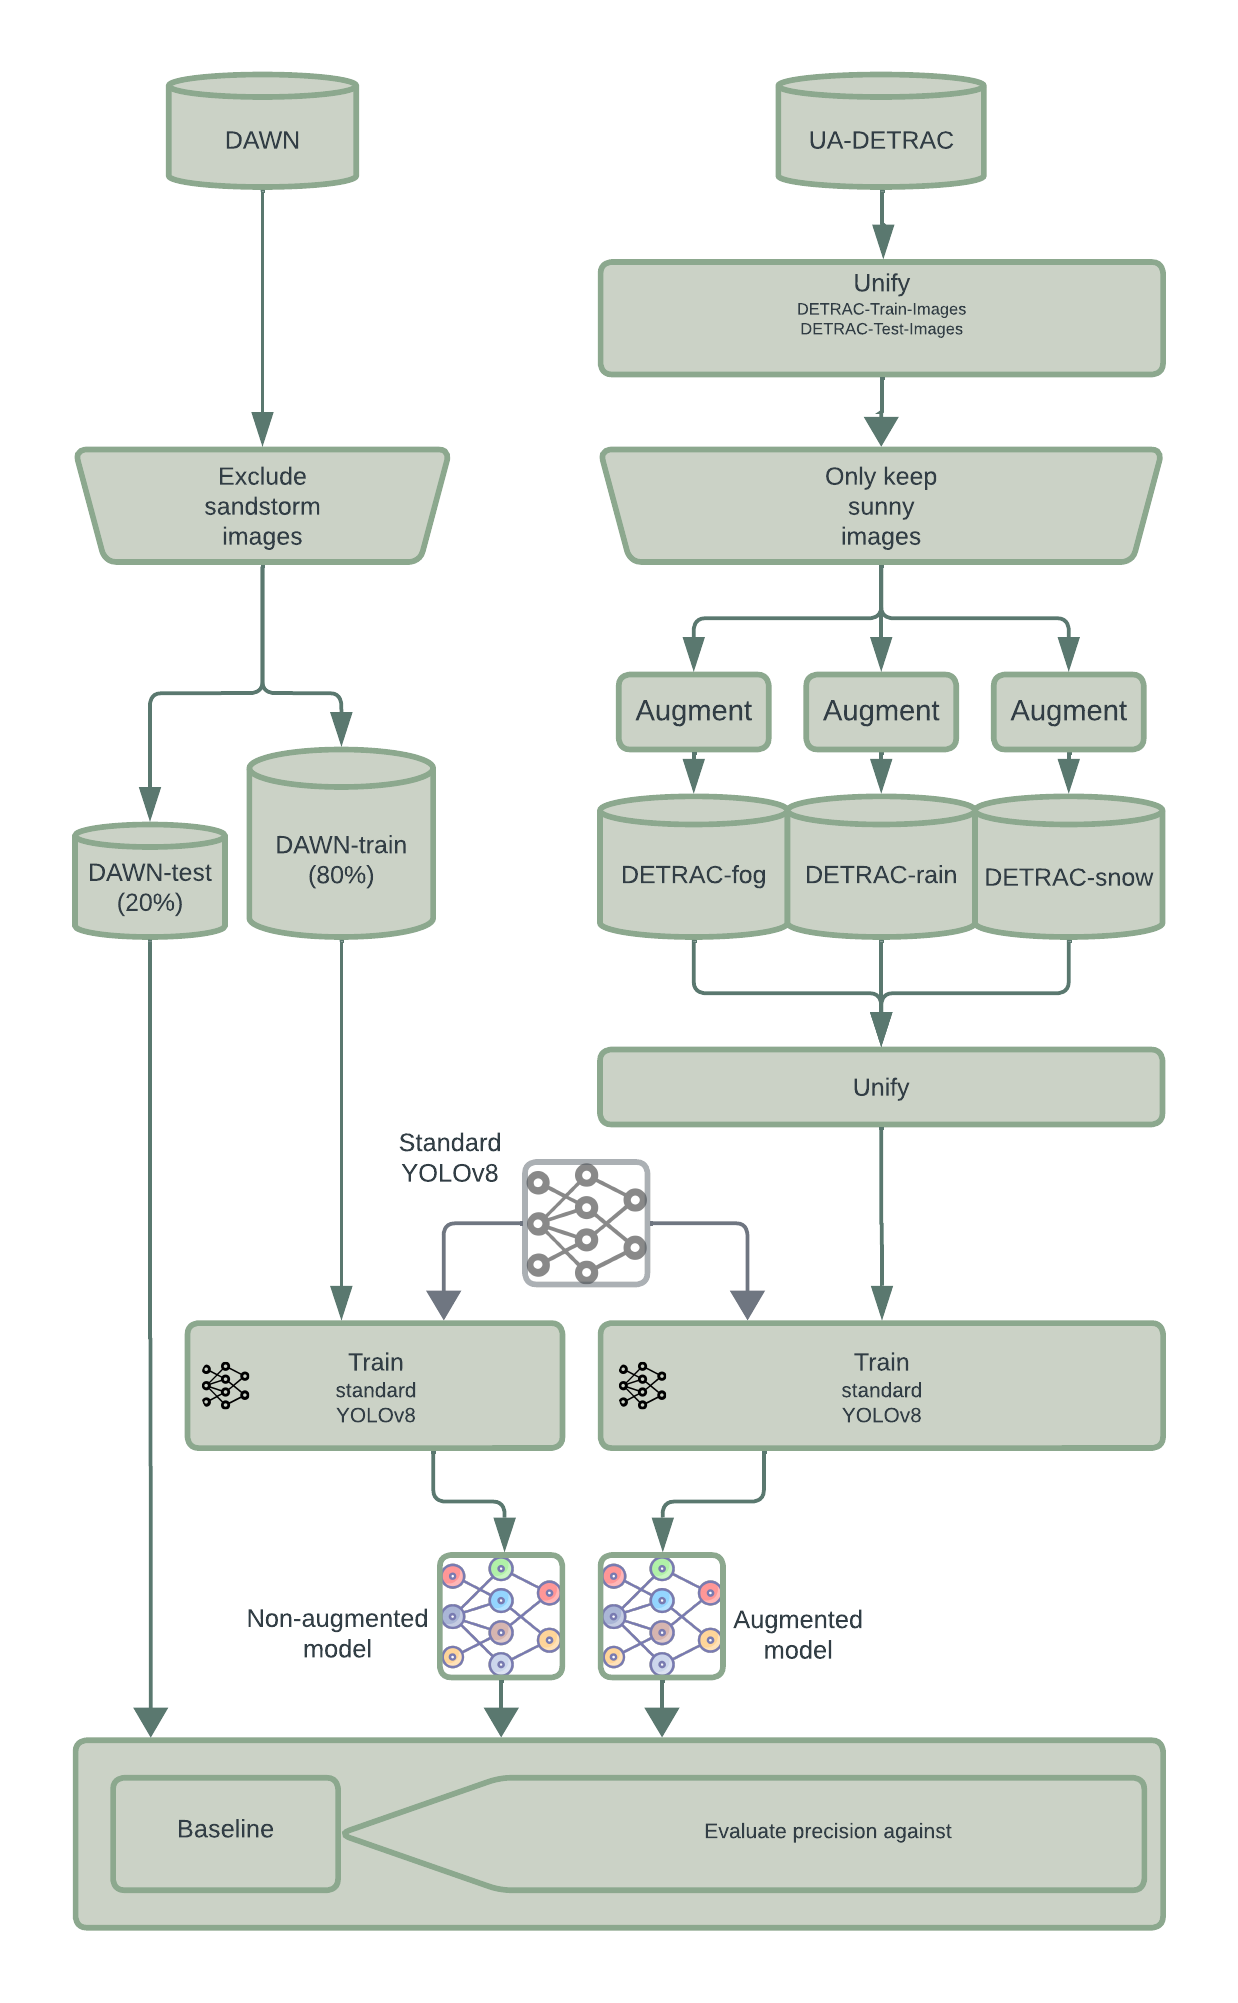
\includegraphics[scale=0.21]{Proposal_diagram.png}
		\caption{Schematic representation of research design}
		\label{fig:experiment_process}
	\end{figure}


\subsection{YOLOv8}

	For vehicle detection we chose YOLO{\small v8}. YOLO is an acronym for ``You Only Look Once'' and denotes a series of models for object detection, image classification, and instance segmentation. The first version of YOLO was released in 2015 by Joseph Redmond. The current standard YOLO{\small v8} model was released in 2023 and is developed and maintained by Ultralytics (\cite{yolov8_ultralytics}). YOLO{\small v8} is based on a deep convolutional neural network architecture and is trained on the Microsoft COCO dataset (\cite{linMicrosoftCOCOCommon2015a}). Since the standard YOLO{\small v8} model is capable of detecting object categories ``car'' and ``bus'', it is fit to serve as a reference model in the proposed research. To refine the standard YOLO{\small v8}  model by transfer learning we envision to use services from roboflow.com.  

\subsection{Data collection}

	Two open-source datasets are used for this research. The smaller one is DAWN and the larger one is UA-DETRAC.

\subsubsection{DAWN}

	The DAWN dataset described in \cite{bw1x-yh39-20}, is a collection of 1000 images of actual traffic events in adverse weather conditions. The images are divided into four equally sized sets of weather conditions: fog, snow, rain and sandstorms. They are labelled according to the categories relevant for current research (``car'' and ``bus'') and annotated with object bounding boxes. From DAWN we exclude all images of wheather type ``sandstorms'' since these do not match with any of our thematic augmentations. We use the remaining image set of 750 images for both validation and training. In particular, the remaining image set is randomly partitioned with a 80/20 ratio. The larger part is denoted by DAWN-train and contains 600 images. The smaller part is denoted by DAWN-test and contains 150 images.

\subsubsection{UA-DETRAC}

	The UA-DETRAC dataset is described in \cite{CVIU_UA-DETRAC}. This dataset provides 140K traffic images taken at 24 different locations in Beijing and Tianjin (China). Images of the UA-DETRAC dataset belong to one of four weather categories: ``cloudy'', ``night'', ``sunny'' and ``rainy''. They are labelled ``car'', ``bus'', ``van'' and ``others''; and annotated with object bounding boxes. The dataset is made available in two parts, a training dataset (DETRAC-Train-Images) and an evaluation dataset (DETRAC-Test-Images). To increase variation in our training set, we use the union of both the DETRAC-Train-Images and DETRAC-Test-Images. From this union we only use images of category ``sunny'', so that the effect of image augmentation is not confounded by images that already showed what the augmentation is adding artificially (eg. augmenting ``cloudy'' or ``rainy'' images with artificial fog or rain). We denote the so obtained set of images by DETRAC-sunny. Finally, to keep consumption of resources (computational and human-hours) within reasonable bounds, we further constrain the volume of images by randomly selecting 200 images from DETRAC-sunny. Table \ref{table:datasets} gives a summary.

	\begin{table}[H]
		\centering
		\begin{tabular}{lccr}
			\toprule
			\textbf{dataset} & \textbf{labels} & \textbf{weather} & \textbf{images} \\
			\midrule
			\textbf{DAWN-train} & car, bus & fog, snow, rain &  600 \\
			\textbf{DAWN-test} & car, bus & fog, snow, rain &  150 \\
			\textbf{DETRAC-sunny} & car, bus & sunny & 200 \\
			\bottomrule
		\end{tabular}
		\caption{The DAWN data sets are not used in image augmentation, they serve as-given for both training and testing. The DETRAC-sunny data set is used in image augmentation and model training.}
		\label{table:datasets}
	\end{table}

\subsection{Image augmentation and training}
	
	To answer research question \ref{rq1} we produce three distinct trainingsets from DETRAC-sunny. One training set is obtained by adding artificial fog, one by adding artificial rain and one by adding artificial snow. The trainingsets are denoted resp. DETRAC-fog, DETRAC-rain and DETRAC-snow and together comprise 600 images. For the image augmentation, we use imgaug \cite{imgaug} (version 0.4.0). We train the standard YOLO{\small v8} model with the union of the DETRAC-fog, DETRAC-rain and DETRAC-snow datasets to produce a new vehicle detection model. This model is referred to as ``the augmented model''. 
	
	To answer research question \ref{rq2} we use the DAWN-train dataset to train the standard YOLO{\small v8} model. This dataset contains 600 actual images of vehicles in adverse weather conditions and since no augmentation is used, the derived model is referred to as ``the non-augmented model''.	A summary of the proposed research is given in tables \ref{table:setuprq1} and \ref{table:setuprq2}.

	\begin{table}[H]
		\centering
		\begin{tabular}{lll}
			\toprule
			\textbf{model} & \textbf{training} & \textbf{testing} \\
			\midrule
			YOLO{\small v8} & none & DAWN-test \\
			\hline
			Augmented model & \begin{tabular}{@{}l@{}}DETRAC-fog \\ DETRAC-rain \\ DETRAC-snow\end{tabular} & DAWN-test \\
			\bottomrule
		\end{tabular}
		\caption{The setup for RQ \ref{rq1} consists in comparing the accuracy of a baseline model with that of an augmented model, given an identical test set DAWN-test.}
		\label{table:setuprq1}
	\end{table}
	
	\begin{table}[H]
		\centering
		\begin{tabular}{lll}
			\toprule
			\textbf{model} & \textbf{training} & \textbf{testing} \\
			\midrule
			YOLO{\small v8} & none & DAWN-test \\
			\hline
			Non-augmented model & DAWN-train & DAWN-test \\
			\bottomrule
		\end{tabular}
		\caption{The setup for RQ \ref{rq2} consists in comparing the accuracy of a baseline model with that of a non-augmented model, given an identical test set DAWN-test.}
		\label{table:setuprq2}
	\end{table}

\section{Data analysis}

	Our approach to the proposed study can best be described as a statistical difference making experiment. We use the mean average precision to rank models by their accuracy in detecting vehicles in images. However, to be more precise about the obtained improvements from refining the standard YOLO{\small v8} model, we propose a hypothesis significance test. 
	
\subsection{Measuring model accuracy}

	To estimate the accuracy of vehicle detection models, we use the mean average precision (mAP) at 0.50-0.95 IoU, henceforth simply referred to as ``mAP''. The mAP is an aggregate metric based on the confusion matrix, the intersection over union (IoU), recall and precision. In this study, we only consider two relevant classes of vehicles, namely ``car'' and ``bus''.

\subsubsection{Calculation of the mAP at 0.50-0.95 IoU}

	The mAP is calculated by dividing the sum of the average precision ($AP$) per class by the number of classes $N$.  In our study $N = 2$ (``car'' and ``bus'').
	
	\[
	mAP = \frac{1}{N} \sum_{i=1}^{N} AP_i
	\]
	
	In summary, the $AP$ of a model is obtained by following steps:
	
	\begin{center}
		\begin{compactenum}
			\item Use model to generate prediction scores
			\item Map prediction scores onto class labels
			\item Construct the confusion matrix
			\item Calculate precision and recall for a set of IoU thresholds (0.50-0.95)
			\item Calculate area under precision-recall curve
			\item Calculate average precision
		\end{compactenum}
	\end{center}
	
	The IoU metric is used to evaluate the performance of object detection by quantifying the fit between the ground truth bounding box and the predicted bounding box.
	
	\begin{figure}[h]
		\centering
		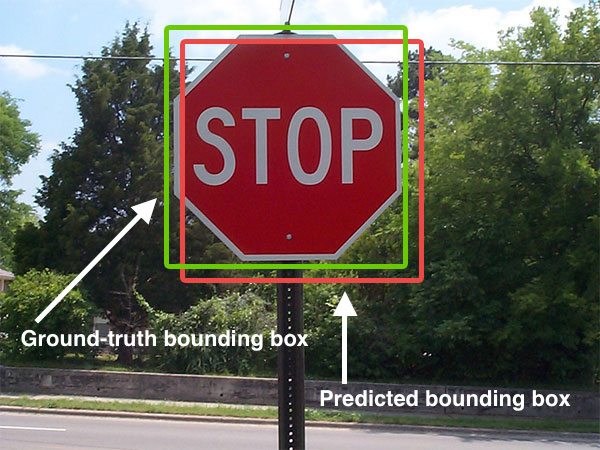
\includegraphics[width=5cm]{Intersection_over_Union_-_object_detection_bounding_boxes.jpg}
		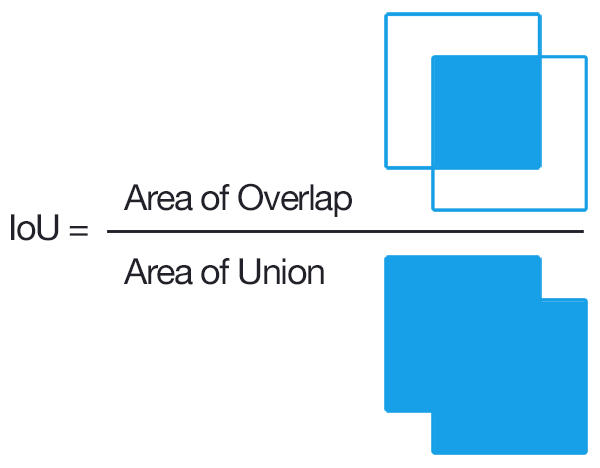
\includegraphics[width=5cm]{Intersection_over_Union_-_visual_equation.png}
		\caption{Illustration of IoU.\\ \footnotesize{(\url{http://www.pyimagesearch.com/2016/11/07/intersection-over-union-iou-for-object-detection/})}}
	\end{figure}
	
	By using a lower bound for the value of the IoU metric, one can discriminate between positive and negative predictions. The IoU metric can then be used to calculate recall and precision. In the context of traffic management, it seems reasonable to favour recall over precision and choose an IoU threshold to reflect this preference. However, choosing a good IoU threshold is itself an optimization process. For comparing models, optimizing the IoU threshold is unnecessary. Instead, we calculate AP as an average of AP's calculated for a set of IoU thresholds per class.
	
\subsubsection{Relevance to proposed research}
	
	From results reported by \cite{kumarObjectDetectionAdverse2023} and \cite{liVehicleDetectionFoggy2022}, we expect to see an improvement in the accuracy of the augmented model as compared with that of the baseline YOLO{\small v8} model. We hold similar expectation for the non-augmented model. More concretely, our scientific hypothesis related to research question \ref{rq1} is that, for the detection of cars and busses in images of traffic in adverse weather conditions, the mAP at 0.50-0.95 IoU of a model obtained by transfer learning from the standard YOLO{\small v8} with thematically augmented images, is higher than that of the standard YOLO{\small v8} model. Our scientific hypothesis related to research question \ref{rq2}, is similar. That is, for the detection of cars and busses in images of traffic in adverse weather conditions, the mAP at 0.50-0.95 IoU of a model obtained by transfer learning from the standard YOLO{\small v8} with  \textit{actual} images, is higher than that of the standard YOLO{\small v8} model.

\subsection{Hypothesis testing}
	
	In light of research question \ref{rq1} we formulate following hypotheses. Define $\mu_1$ as the mean IoU obtained from predictions made by the augmented model over the DAWN-test set, and likewise $\mu_2$ as that obtained from predictions made by the baseline model (YOLO{\small v8}) over the same DAWN-test set. Then, the null hypothesis $H_0$ and alternative hypothesis $H_a$ are given as:
	
	\begin{itemize}
		\item $H_0$: $\mu_1 \le \mu_2$. 
		\item $H_a$: $\mu_1 > \mu_2$
	\end{itemize}
	
	We use a one-tailed t-test to determine if $H_0$ can be rejected at the 0.05 significance level. If this is the case we answer research question \ref{rq1} in the affirmative, which means that training with augmented images indeed yields better accuracy in vehicle detection. 
	
	In light of research question \ref{rq2} we formulate similar hypotheses and reject $H_0$ at the 0.05 significance level. Again, if this is the case we answer \ref{rq2} in the affirmative and take that training with actual images also yields better accuracy in vehicle detection.
	Finally, to answer research question \ref{rq3} we use the ``two one-sided t-test'' (TOST) procedure.

\section{Proposed time line}

The following tasks will have to be addressed (see Figure \ref{fig:timeline}) :
\begin{itemize}
	\item Dataset preparation
	\item Images augmentation
	\item Training models
	\item Evaluation of models
	\item Data analysis
	\item Write the report
\end{itemize}

\begin{figure}[H]
	\centering
	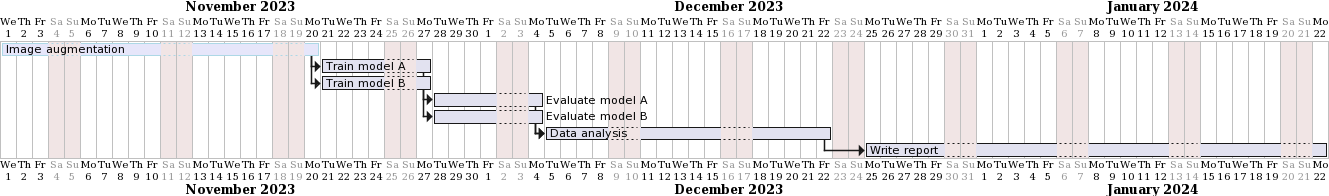
\includegraphics[width=\textwidth]{proposal-timing}
	\caption{Proposed timeline}
	\label{fig:timeline}
\end{figure}

\printbibliography

\end{document}
